\documentclass{article}
\usepackage{graphicx}
\usepackage{amsmath}
\usepackage{fancyhdr}
\usepackage[margin=1in]{geometry}
\usepackage{comment}
\usepackage{placeins}
\usepackage{parskip}
\usepackage{subcaption}
\usepackage{appendix}
\usepackage{soul}
\usepackage{comment}
\usepackage[hidelinks]{hyperref}
\usepackage{matlab-prettifier}
\usepackage{minted}
\usepackage{pdfpages}

\pagestyle{fancy}
\fancyhf{} % Clear header/footer settings
\rhead{\thepage} % Page number on the right in the header
\lhead{ASE375 Lab Report 2} % Your lab report title on the left

\begin{document}

\begin{titlepage}
  \centering
  
\includegraphics[width=10cm]{ase-logo-formal.png}  % Adjust the width as needed
  \vspace{1cm}  % Add some vertical space
 
  \Large \textbf{ASE 375 Electromechanical Systems}\\
  \large \textbf{Section 14115}\\
  \vspace{0.5cm}
  \textbf{Monday: 3:00 - 6:00 pm}\\
 
  \vspace{1cm}
 
  \hrule
  \vspace{0.5cm}
 
  \Huge \textbf{Report 2:\\
  Temperature Sensor Measurements}\\
  \Huge \textbf{}\\
 
  \vspace{0.5cm}
  \hrule
 
  \vspace{1cm}
 
  \normalsize \textbf{Andrew Doty, Andres Suniaga, Dennis Hom}\\
  \normalsize \textbf{Due Date: 02/12/2024}
 
\end{titlepage}
\newpage

\tableofcontents
\thispagestyle{empty}
\newpage



\section{Introduction}
This experiment consisted of measuring temperature with three different sensors: a Thermocouple, Thermistor, and an Integrated Circuit Temperature sensor. Data collection was made possible through a Data Acquisition (DAQ) system used to process the different temperature measurements in LabVIEW, a graphical interface that modeled the temperature sensors' measurements. 

The purpose of this experiment was to learn how to simulate our data through LabVIEW along with observing and understanding the behaviour of the three temperature sensors in different environments: $(1)$ at room temperature, $(2)$ in water near freezing conditions, and $(3)$ in water closer to boiling conditions. 

\section{Equipment}
The equipment used in this experiment include .....

K-type Thermocouple:  connected to NI 9211

Thermistor:  connected to NI 9215 via breadboard w/ 1k ohm resistor etc....

IC Temperature Sensor: connected to NI 9215

Breadboard: 

Circuit Components:  various male-to-male jumper wires, $1k\;\Omega$ resistor, etc... and 5V power supply

DAQ:  Data Aquisition system that digitizes analog information into "bins" for a computer.  The specific DAQ had two units, the NI 9215 and NI 9211.  Specific Datasheets for each are included in the appendices.  

Thermometer:  used to measure true temperature w/ 0.5 degrees 

Water:  Access to water near a boiling temperature, and water in an ice bath.   




\section{Procedure}


\section{Data Processing}

\subsection{Part 1}


\subsection{Part 2}


\section{Results and Analysis}



\section{Conclusion}




\newpage
\thispagestyle{empty}  % Clear header/footer
\begin{center}
	\vspace*{\fill}
	{\Huge Appendices}
	\vspace*{\fill}
\end{center}

% Start appendices
\newpage
\begin{appendices}
\pagestyle{fancy}
\renewcommand{\thefigure}{A\arabic{figure}}
\setcounter{figure}{0}

\section*{Appendix: t-Distribution Tables}
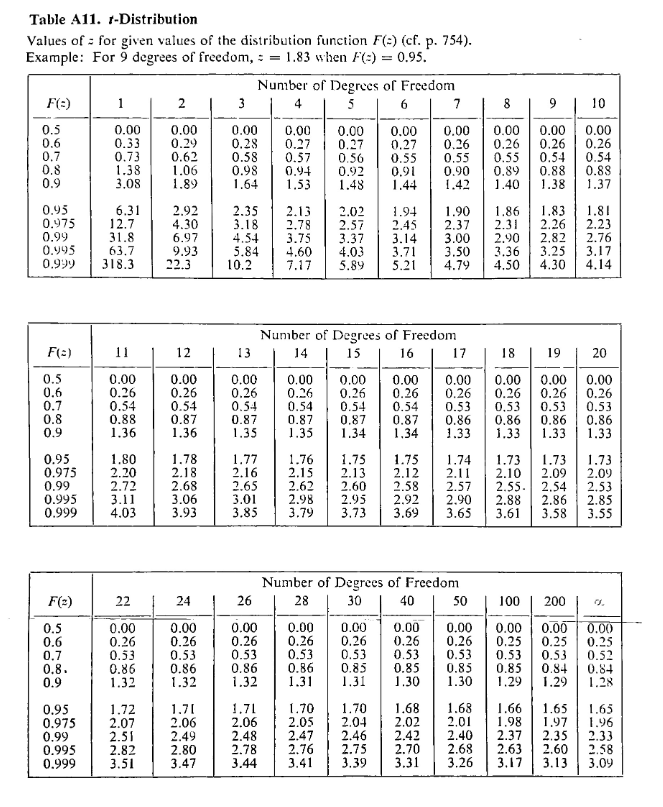
\includegraphics[width=\textwidth]{t_distribution_Table_lecture3.png}
\end{appendices}


\end{document}






